\documentclass{standalone}
\usepackage{tikz}
\usetikzlibrary{patterns, positioning}

\begin{document}
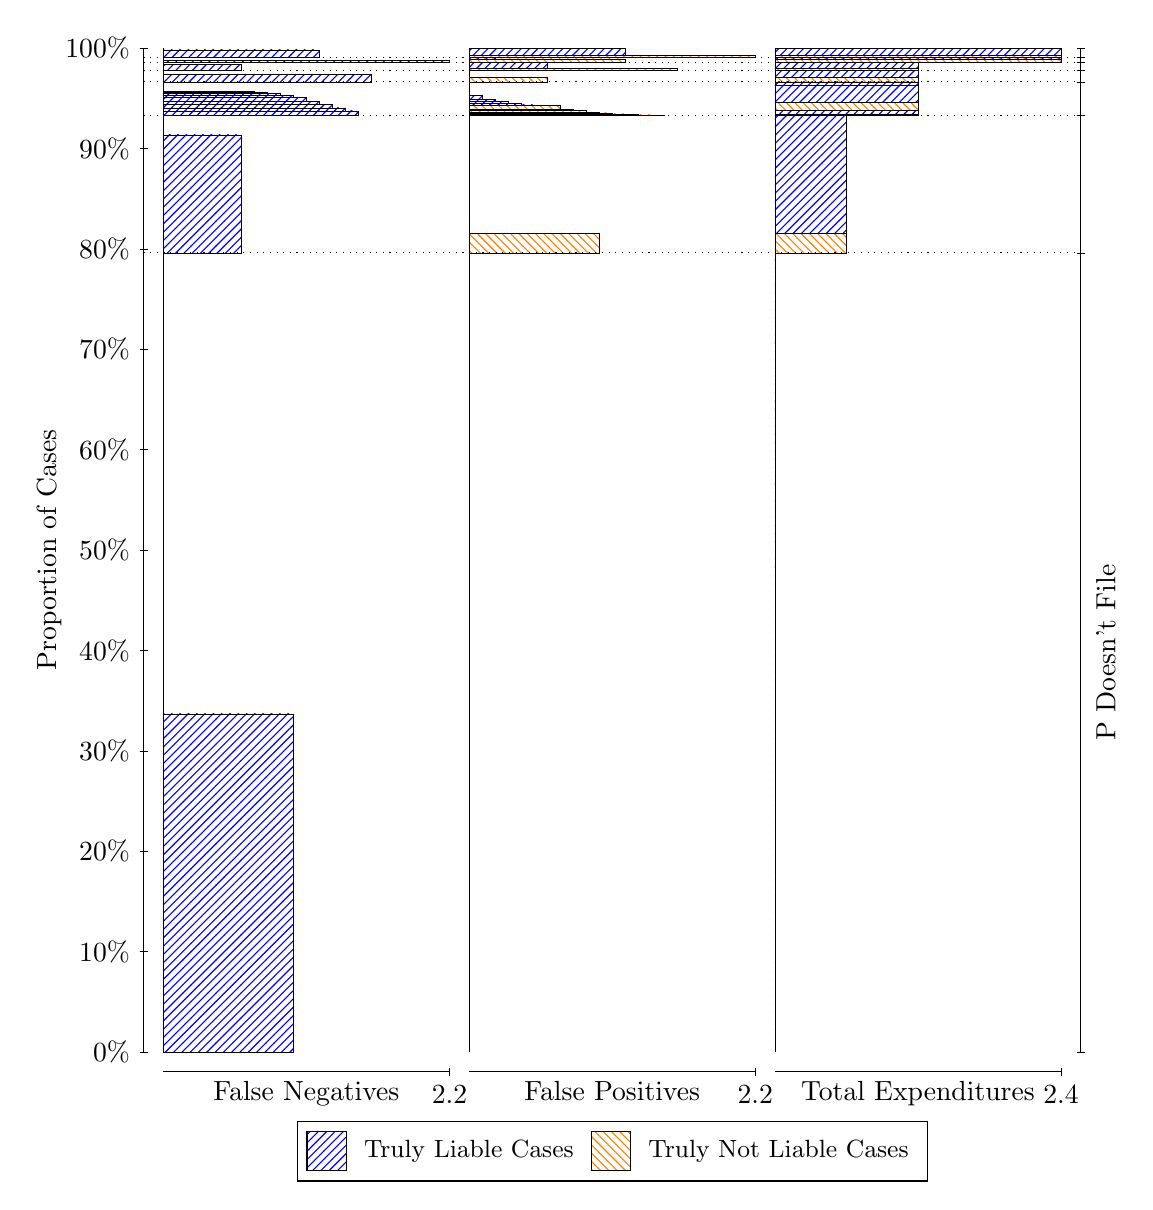
\begin{tikzpicture}
\draw[black, very thin] (1.5,1.75) -- (1.5,14.5);
\node[rotate=90, anchor=center] at (0.3, 8.125) {Proportion of Cases};
\draw[black, very thin] (1.45,1.75) -- (1.55,1.75);
\node[anchor=east] at (1.45, 1.75) {0\%};
\draw[black, very thin] (1.45,3.025) -- (1.55,3.025);
\node[anchor=east] at (1.45, 3.025) {10\%};
\draw[black, very thin] (1.45,4.3) -- (1.55,4.3);
\node[anchor=east] at (1.45, 4.3) {20\%};
\draw[black, very thin] (1.45,5.575) -- (1.55,5.575);
\node[anchor=east] at (1.45, 5.575) {30\%};
\draw[black, very thin] (1.45,6.85) -- (1.55,6.85);
\node[anchor=east] at (1.45, 6.85) {40\%};
\draw[black, very thin] (1.45,8.125) -- (1.55,8.125);
\node[anchor=east] at (1.45, 8.125) {50\%};
\draw[black, very thin] (1.45,9.4) -- (1.55,9.4);
\node[anchor=east] at (1.45, 9.4) {60\%};
\draw[black, very thin] (1.45,10.675) -- (1.55,10.675);
\node[anchor=east] at (1.45, 10.675) {70\%};
\draw[black, very thin] (1.45,11.95) -- (1.55,11.95);
\node[anchor=east] at (1.45, 11.95) {80\%};
\draw[black, very thin] (1.45,13.225) -- (1.55,13.225);
\node[anchor=east] at (1.45, 13.225) {90\%};
\draw[black, very thin] (1.45,14.5) -- (1.55,14.5);
\node[anchor=east] at (1.45, 14.5) {100\%};

\draw[black, very thin] (13.4,1.75) -- (13.4,14.5);
\draw[black, very thin] (13.35,1.75) -- (13.45,1.75);
\node[anchor=west] at (13.35, 1.75) {};
\draw[black, very thin] (13.35,11.898) -- (13.45,11.898);
\node[anchor=west] at (13.35, 11.898) {};
\draw[black, very thin] (13.35,13.644) -- (13.45,13.644);
\node[anchor=west] at (13.35, 13.644) {};
\draw[black, very thin] (13.35,14.071) -- (13.45,14.071);
\node[anchor=west] at (13.35, 14.071) {};
\draw[black, very thin] (13.35,14.215) -- (13.45,14.215);
\node[anchor=west] at (13.35, 14.215) {};
\draw[black, very thin] (13.35,14.318) -- (13.45,14.318);
\node[anchor=west] at (13.35, 14.318) {};
\draw[black, very thin] (13.35,14.384) -- (13.45,14.384);
\node[anchor=west] at (13.35, 14.384) {};
\draw[black, very thin] (13.35,14.5) -- (13.45,14.5);
\node[anchor=west] at (13.35, 14.5) {};

\draw[black, very thin, pattern color=blue, pattern=north east lines] (1.75,1.75) rectangle (3.4015,6.0433);
\draw[black, very thin, pattern color=orange, pattern=north west lines] (1.75,6.0433) rectangle (1.75,11.898);
\draw[black, very thin, pattern color=blue, pattern=north east lines] (1.75,11.898) rectangle (2.7409,13.396);
\draw[black, very thin, pattern color=orange, pattern=north west lines] (1.75,13.396) rectangle (1.75,13.644);
\draw[black, very thin, pattern color=blue, pattern=north east lines] (1.75,13.644) rectangle (4.2273,13.703);
\draw[black, very thin, pattern color=blue, pattern=north east lines] (1.75,13.703) rectangle (4.0621,13.74);
\draw[black, very thin, pattern color=blue, pattern=north east lines] (1.75,13.74) rectangle (3.897,13.788);
\draw[black, very thin, pattern color=blue, pattern=north east lines] (1.75,13.788) rectangle (3.7318,13.821);
\draw[black, very thin, pattern color=blue, pattern=north east lines] (1.75,13.821) rectangle (3.5667,13.869);
\draw[black, very thin, pattern color=blue, pattern=north east lines] (1.75,13.869) rectangle (3.4015,13.895);
\draw[black, very thin, pattern color=blue, pattern=north east lines] (1.75,13.895) rectangle (3.2364,13.923);
\draw[black, very thin, pattern color=blue, pattern=north east lines] (1.75,13.923) rectangle (3.0712,13.937);
\draw[black, very thin, pattern color=blue, pattern=north east lines] (1.75,13.937) rectangle (2.9061,13.948);
\draw[black, very thin, pattern color=orange, pattern=north west lines] (1.75,13.948) rectangle (1.75,14.071);
\draw[black, very thin, pattern color=blue, pattern=north east lines] (1.75,14.071) rectangle (4.3924,14.161);
\draw[black, very thin, pattern color=orange, pattern=north west lines] (1.75,14.161) rectangle (1.75,14.215);
\draw[black, very thin, pattern color=blue, pattern=north east lines] (1.75,14.215) rectangle (2.7409,14.291);
\draw[black, very thin, pattern color=orange, pattern=north west lines] (1.75,14.291) rectangle (1.75,14.318);
\draw[black, very thin, pattern color=blue, pattern=north east lines] (1.75,14.318) rectangle (5.3833,14.342);
\draw[black, very thin, pattern color=orange, pattern=north west lines] (1.75,14.342) rectangle (1.75,14.384);
\draw[black, very thin, pattern color=blue, pattern=north east lines] (1.75,14.384) rectangle (3.7318,14.476);
\draw[black, very thin, pattern color=orange, pattern=north west lines] (1.75,14.476) rectangle (1.75,14.5);
\draw[black, very thin, pattern color=orange, pattern=north west lines] (5.6333,1.75) rectangle (5.6333,7.6045);
\draw[black, very thin, pattern color=blue, pattern=north east lines] (5.6333,7.6045) rectangle (5.6333,11.898);
\draw[black, very thin, pattern color=orange, pattern=north west lines] (5.6333,11.898) rectangle (7.2848,12.146);
\draw[black, very thin, pattern color=blue, pattern=north east lines] (5.6333,12.146) rectangle (5.6333,13.644);
\draw[black, very thin, pattern color=orange, pattern=north west lines] (5.6333,13.644) rectangle (8.1106,13.647);
\draw[black, very thin, pattern color=orange, pattern=north west lines] (5.6333,13.647) rectangle (7.9455,13.65);
\draw[black, very thin, pattern color=orange, pattern=north west lines] (5.6333,13.65) rectangle (7.7803,13.656);
\draw[black, very thin, pattern color=orange, pattern=north west lines] (5.6333,13.656) rectangle (7.6152,13.663);
\draw[black, very thin, pattern color=orange, pattern=north west lines] (5.6333,13.663) rectangle (7.45,13.676);
\draw[black, very thin, pattern color=orange, pattern=north west lines] (5.6333,13.676) rectangle (7.2848,13.685);
\draw[black, very thin, pattern color=orange, pattern=north west lines] (5.6333,13.685) rectangle (7.1197,13.704);
\draw[black, very thin, pattern color=orange, pattern=north west lines] (5.6333,13.704) rectangle (6.9545,13.721);
\draw[black, very thin, pattern color=orange, pattern=north west lines] (5.6333,13.721) rectangle (6.7894,13.767);
\draw[black, very thin, pattern color=blue, pattern=north east lines] (5.6333,13.767) rectangle (6.4591,13.779);
\draw[black, very thin, pattern color=blue, pattern=north east lines] (5.6333,13.779) rectangle (6.2939,13.792);
\draw[black, very thin, pattern color=blue, pattern=north east lines] (5.6333,13.792) rectangle (6.1288,13.82);
\draw[black, very thin, pattern color=blue, pattern=north east lines] (5.6333,13.82) rectangle (5.9636,13.846);
\draw[black, very thin, pattern color=blue, pattern=north east lines] (5.6333,13.846) rectangle (5.7985,13.894);
\draw[black, very thin, pattern color=blue, pattern=north east lines] (5.6333,13.894) rectangle (5.6333,14.071);
\draw[black, very thin, pattern color=orange, pattern=north west lines] (5.6333,14.071) rectangle (6.6242,14.126);
\draw[black, very thin, pattern color=blue, pattern=north east lines] (5.6333,14.126) rectangle (5.6333,14.215);
\draw[black, very thin, pattern color=orange, pattern=north west lines] (5.6333,14.215) rectangle (8.2758,14.243);
\draw[black, very thin, pattern color=blue, pattern=north east lines] (5.6333,14.243) rectangle (6.6242,14.318);
\draw[black, very thin, pattern color=orange, pattern=north west lines] (5.6333,14.318) rectangle (7.6152,14.361);
\draw[black, very thin, pattern color=blue, pattern=north east lines] (5.6333,14.361) rectangle (5.9636,14.384);
\draw[black, very thin, pattern color=orange, pattern=north west lines] (5.6333,14.384) rectangle (9.2667,14.409);
\draw[black, very thin, pattern color=blue, pattern=north east lines] (5.6333,14.409) rectangle (7.6152,14.5);
\draw[black, very thin, pattern color=orange, pattern=north west lines] (9.5167,1.75) rectangle (9.5167,7.6045);
\draw[black, very thin, pattern color=blue, pattern=north east lines] (9.5167,7.6045) rectangle (9.5167,11.898);
\draw[black, very thin, pattern color=orange, pattern=north west lines] (9.5167,11.898) rectangle (10.425,12.146);
\draw[black, very thin, pattern color=blue, pattern=north east lines] (9.5167,12.146) rectangle (10.425,13.644);
\draw[black, very thin, pattern color=orange, pattern=north west lines] (9.5167,13.644) rectangle (11.333,13.657);
\draw[black, very thin, pattern color=blue, pattern=north east lines] (9.5167,13.657) rectangle (11.333,13.705);
\draw[black, very thin, pattern color=orange, pattern=north west lines] (9.5167,13.705) rectangle (11.333,13.807);
\draw[black, very thin, pattern color=blue, pattern=north east lines] (9.5167,13.807) rectangle (11.333,14.021);
\draw[black, very thin, pattern color=orange, pattern=north west lines] (9.5167,14.021) rectangle (11.333,14.03);
\draw[black, very thin, pattern color=blue, pattern=north east lines] (9.5167,14.03) rectangle (11.333,14.071);
\draw[black, very thin, pattern color=orange, pattern=north west lines] (9.5167,14.071) rectangle (11.333,14.126);
\draw[black, very thin, pattern color=blue, pattern=north east lines] (9.5167,14.126) rectangle (11.333,14.215);
\draw[black, very thin, pattern color=orange, pattern=north west lines] (9.5167,14.215) rectangle (11.333,14.243);
\draw[black, very thin, pattern color=blue, pattern=north east lines] (9.5167,14.243) rectangle (11.333,14.318);
\draw[black, very thin, pattern color=orange, pattern=north west lines] (9.5167,14.318) rectangle (13.15,14.361);
\draw[black, very thin, pattern color=blue, pattern=north east lines] (9.5167,14.361) rectangle (13.15,14.384);
\draw[black, very thin, pattern color=orange, pattern=north west lines] (9.5167,14.384) rectangle (13.15,14.409);
\draw[black, very thin, pattern color=blue, pattern=north east lines] (9.5167,14.409) rectangle (13.15,14.5);
\draw[black, dotted] (1.5,11.898) -- (13.4,11.898);
\draw[black, dotted] (1.5,13.644) -- (13.4,13.644);
\draw[black, dotted] (1.5,14.071) -- (13.4,14.071);
\draw[black, dotted] (1.5,14.215) -- (13.4,14.215);
\draw[black, dotted] (1.5,14.318) -- (13.4,14.318);
\draw[black, dotted] (1.5,14.384) -- (13.4,14.384);
\draw[black, very thin] (1.75,1.5) -- (5.3833,1.5);
\node[anchor=north] at (3.5667, 1.5) {False Negatives};
\draw[black, very thin] (5.3833,1.45) -- (5.3833,1.55);
\node[anchor=north] at (5.3833, 1.45) {2.2};

\draw[black, very thin] (5.6333,1.5) -- (9.2667,1.5);
\node[anchor=north] at (7.45, 1.5) {False Positives};
\draw[black, very thin] (9.2667,1.45) -- (9.2667,1.55);
\node[anchor=north] at (9.2667, 1.45) {2.2};

\draw[black, very thin] (9.5167,1.5) -- (13.15,1.5);
\node[anchor=north] at (11.333, 1.5) {Total Expenditures};
\draw[black, very thin] (13.15,1.45) -- (13.15,1.55);
\node[anchor=north] at (13.15, 1.45) {2.4};

\node[black, centered, rotate=90] at (13.72, 6.8239) {P Doesn't File};







\draw (7.449999999999999,1.5) node[draw=none] (baseCoordinate) {};
\begin{scope}[align=center]
        \matrix[scale=0.5, draw=black, below=0.5cm of baseCoordinate, nodes={draw}, column sep=0.1cm]{
            \node[rectangle, draw, minimum width=0.5cm, minimum height=0.5cm, pattern=north east lines, pattern color=blue] {}; &
            \node[draw=none, font=\small] (B) {Truly Liable Cases}; &
            \node[rectangle, draw, minimum width=0.5cm, minimum height=0.5cm, pattern=north west lines, pattern color=orange] {}; &
            \node[draw=none, font=\small] (B) {Truly Not Liable Cases}; \\
            };
\end{scope}

\end{tikzpicture}
\end{document}